\documentclass{sbir}

%\usepackage{fixme}
%\fxsetup{
%    status=draft,
%    author=,
%    layout=margin,
%    theme=color,
%    targetlayout=color
%}

%%%%%%%%%% Proposal-specific Information %%%%%%%%%%%%%%%
\company{Modus Operandi}
\proposaltitle{GeoAID: Geographically-aware Assured Information Dissemination}
\topicnum{AF131-039}
\proposalnum{F131-039-0974}
\proposaltype{SBIR Phase I Proposal}
%%%%%%%%%%%%%%%%%%%%%%%%%%%%%%%%%%%%%%%%

\begin{document}

%\listoffixmes
%\newpage
 
%%%%%  Roman numerals for TOC  %%%%%
\pagenumbering{roman}
\tableofcontents
\newpage
 
%%%%% Set the page number that the main proposal will start on %%%%%%
\pagenumbering{arabic}
\pagestyle{proprietary}

\cfoot{
{\color{LeTigre}\vspace*{-1.1in}{\it\small{This proposal includes data that shall not be disclosed outside the Government and shall not be duplicated, used, or disclosed-in whole or in part-for any purpose other than to evaluate this proposal. If, however, a contract is awarded to this offeror as a result of-or in connection with-the submission of this data, the Government shall have the right to duplicate, use, or disclose the data to the extent provided in the resulting contract. This restriction does not limit the Government's right to use information contained in this data if it is obtained from another source without restriction. The data subject to this restriction are contained in pages 1--5 and 7--20.}~\\
\scshape\fromproposaltitle}~\\ \rm\thepage }
}

\sbirsection{Identification and Significance of the Problem or Opportunity}
{The Modus Operandi Team proposes to develop geographically-aware assured information dissemination system called GeoAID. This system will leverage our expertise and ongoing work in the areas of usage management and policy-based assured information sharing in network-centric multilevel security environments. The ability of GeoAID to rapidly and dynamically provide assured information and services to targeted devices within specific geographic regions will produce an information advantage for warfighters, and has direct commercial applicability to the emergency response industry.}

%%%%%  Evaluation Criteria box, use \begin{evalbox} \end{evalbox}, \evalhdr, \begin{evalitemize}, and \end{evalitemize}  %%%%% 	
\begin{evalbox}
\evalhdr{Innovative:}
  \begin{evalitemize}
     \item Addresses the GATSID problem via a proven policy-based usage management framework.
     \item Naturally incorporates location-based access policies into broader usage policies.
     \item Underlying logic framework supports sophisticated formal reasoning capabilities.
  \end{evalitemize}
\evalhdr{Sound Technical Approach:}
  \begin{evalitemize}
     \item Based on open standards and GOTS product development.
     \item Leverages UNM's demonstrated work in policy-based usage management.
     \item Leverages MO's proven work in defense software systems development.
  \end{evalitemize}
\evalhdr{Qualifications:}
  \begin{evalitemize}
     \item MO Co-PI has significant experience with SBIR/STTR development and technology transition.
     \item AHS Co-PI has considerable expertise in information security and usage management.
  \end{evalitemize}
\evalhdr{Benefits:}
  \begin{evalitemize}
     \item Dynamically and securely share information with properly credentialed users based upon location.
     \item An agile usage management framework that scales to the enterprise.
     \item Provides an information advantage to warfighters.
  \end{evalitemize}
\evalhdr{Commercialization:}
  \begin{evalitemize}
     \item Deployable in any networked environment where location-based usage policies apply.
  \end{evalitemize}
\end{evalbox}

\paragraph{Executive Summary}
\paragraph{The Problem.} The goal of this research and development effort is to build a system that addresses the Geographically-Aware and Targeted Secure Information Dissemination (GATSID) problem. In the GATSID problem, the warfighter is assumed to possess an Internet Protocol (IP)-based wireless device (or set of devices) that may connect to the military Internet. Furthermore, some collection of the devices associated with the network is assumed to support position location capabilities via a Global Positioning System (GPS). Given these assumptions, the goal is to build a system that ``will enable on-the-move warfighters \ldots to securely send and receive information that can be targeted and tailored for sender-specified regions, sectors, or operating areas~\cite{AF131-039}.'' Given such a system, there are numerous scenarios (some of which are described below) where its capabilities could be leveraged to provide a distinct information advantage to the warfighter in the field.

However, there are numerous difficulties with this approach that must be accounted for by any system deployed to address the GATSID problem. Most importantly, all advantages to the warfighter may be lost if information is not delivered in a provably assured manner. Indeed, we can easily conceive of mission scenarios where opposing forces actually gain strategic advantage due to information leakage associated with an improperly designed location-based dissemination system. It would not be difficult to build a system that addresses the GATSID problem if we could hold all aspects of the operating and mission environments constant. In this case, a set of rules for how and when information should be delivered to whom could be enumerated and exhaustively validated. The reality, however, is that military network environments are constantly changing in ways that cannot be anticipated, and no two mission environments are the same. Thus, an architectural framework that is overly rigid will lead to a system that cannot be easily adapted or scaled to address future needs. It is not uncommon for the complexity of such systems to grow over time, leading to a security situation that becomes increasingly more difficult to manage.

\clearpage
\cfoot{\color{LeTigre}\vspace*{-1.25em}{\scshape\fromproposaltitle}~\\ \rm\thepage~\\ 
\it{Use or disclosure of data contained on this page is subject to the restriction on the first page of this volume.}}

\paragraph{The Solution Objective.} The Modus Operandi Team, composed of Modus Operandi, Inc. (MO) and AHS Engineering Services (AHS), proposes to design, prototype, and develop the Geographically-aware Assured Information Dissemination (GeoAID) system for addressing the GATSID problem. The GeoAID system will be built on top of a highly flexible usage management framework that was designed to address situations very similar to GATSID, and was built with the notion of operating in Internet-scale environments involving highly complex usage policies.

\paragraph{Our Approach.} The proposed research addresses the problem described above by logically separating security policies from security implementations within the network. This approach is vital if the true capabilities of GATSID are to be realized in DoD environments. In a DoD setting there will be multiple missions currently interacting with the network infrastructure, and the proposed framework will allow each mission to do so according to the current security policies. Our approach will leverage our extensive information security work in policy-based usage management. Figure~\ref{conops} provides a high level view of the GeoAID concept of operations. The key element to note in this figure is the manner in which usage management capabilities are deployed throughout the infrastructure---at the distribution network, at nodes within a hierarchal geographically local network~(Network I), and as a part of each node in an ad-hoc geographically local network~(Network II). A \emph{policy decision point} is assumed at the headquarters in this figure. From this point, messages along with bound polices can be created for distribution, e.g.,  through a banner-in-the-sky (BitS) service. The usage management subsystems, a capability we have spent numerous years developing and maturing, provide \emph{policy enforcement points} at critical locations within the networking environment. For instance, at the Distribution Network we have  demonstrated the capability of redacting message content or re-routing based upon dynamically evaluated policies. The figure also shows two scenarios, one~(red arrows) in which a message flows from the BitS to all nodes in one local network, and then to the nodes in an adjacent local network via a policy-mediated multicast mechanism. In the second scenario (blue arrows), usage management policies constrain a message to in-theater nodes.

%The key elements to note in this figure are the policy-based nature of our approach, the manner in which usage policy is given meaning via an ontology, and the fact that usage policy is always interpreted relative to the current context of the user. More specifically, on the left side of this figure, in Domain A, usage policy is first transformed into a license, using the ontology that has been defined for the particular usage management environment that the system will be operating in. Next, the license is bound to a particular resource, and this bundle is the element that is then made available for usage-managed sharing in other domains.

\paragraph{Vision and End-State.} The end state of our Phase I research project will be the production of the GeoAID architecture and initial prototype that demonstrate the feasibility of our approach for success during Phases II and III. Specifically the prototype will demonstrate a means to collect and identify potential receiving nodes by class, location, or other means, and will provide assured information dissemination to these nodes. The \emph{technology readiness level} will be established at the conclusion of Phase I.

\paragraph{Background and Need}~\\
On the move warfighters require access to relevant, geo-tagged information. This information must be delivered to devices including handheld multi-function computers, either commercially available or militarized, or wearable computational systems incorporating novel user interface schemes.

\begin{figure}
\vspace{-0.2in}
  \centerline{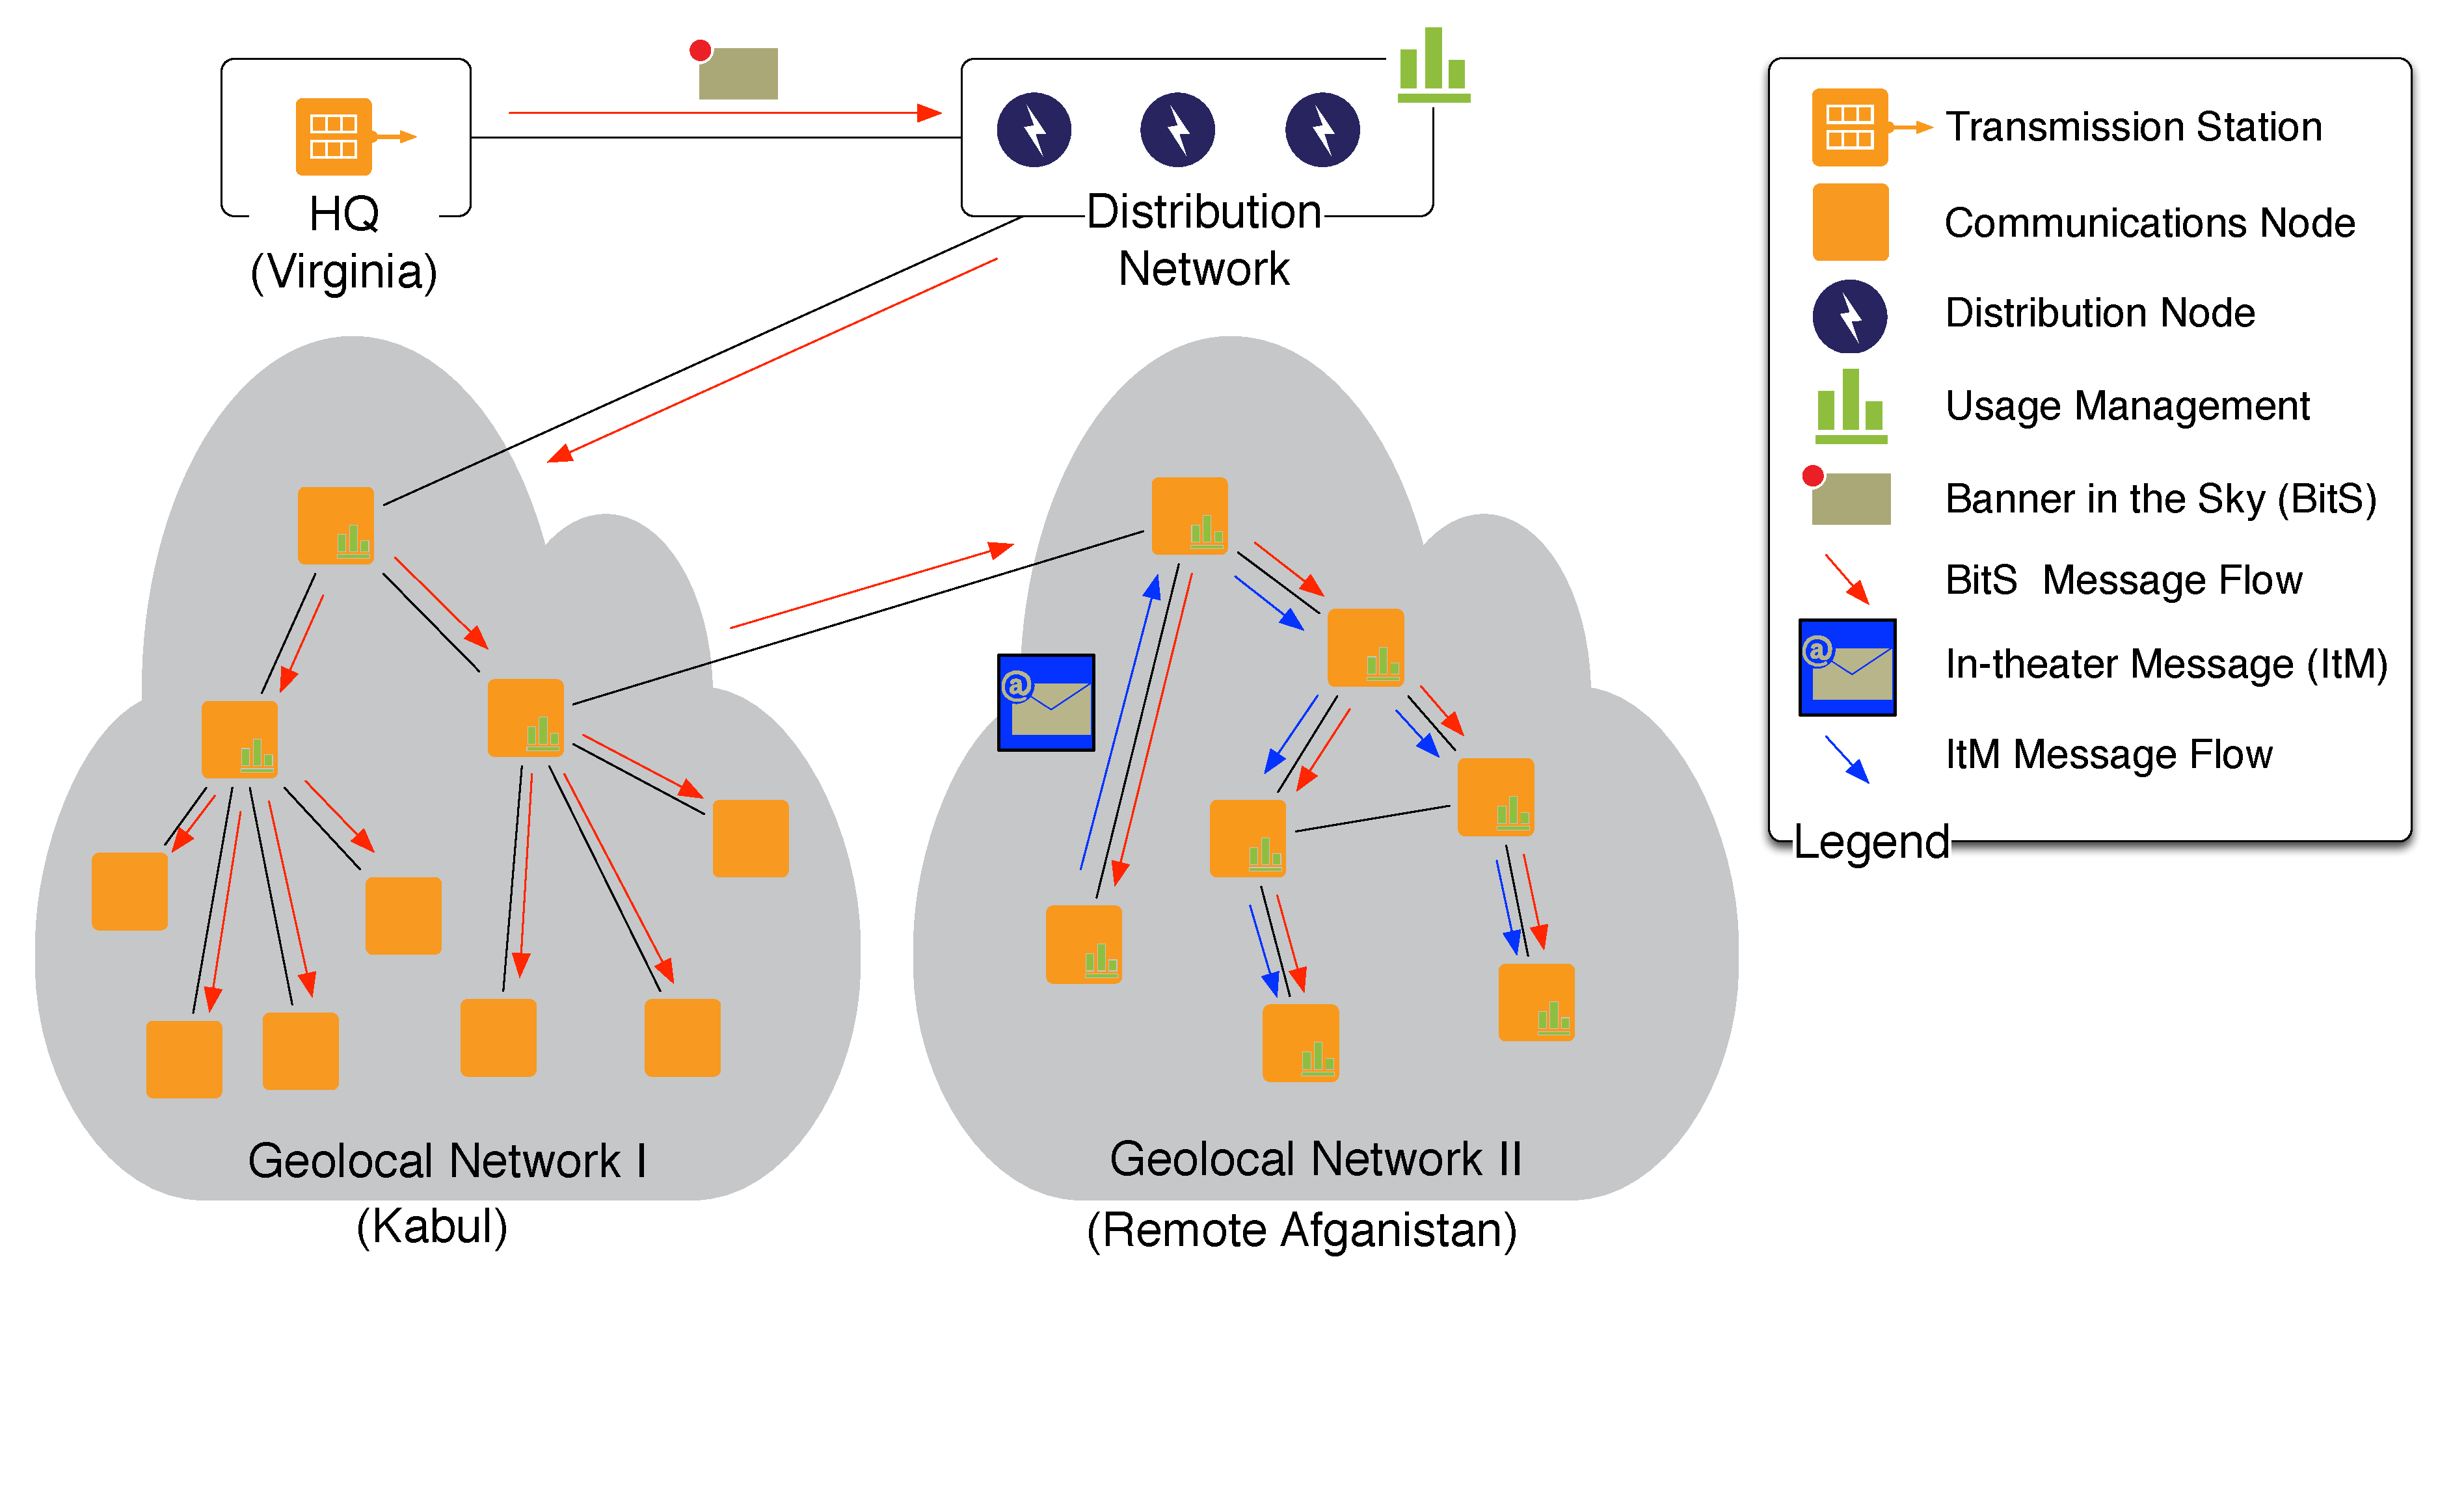
\includegraphics[width=5in]{./images/conops-gatsid.pdf}}
    \vspace{-0.1in}
  \caption{The concept of operations for the GeoAID system.}
  \label{conops}
\end{figure}


%\begin{figure}
%  \centerline{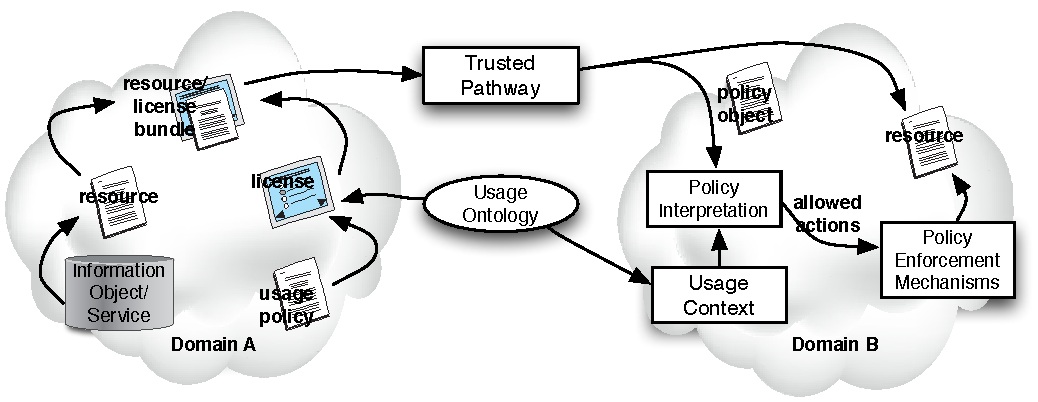
\includegraphics[width=5.5in]{./images/UM-highlevel.pdf}}
%  \caption{A high level depiction of the usage management framework.}
%  \label{UM-highlevel}
% \end{figure}

\sbircallout{The technical challenges.}{Current systems provide static, one-size-fits-all functionality for operational information delivery. This is unsuitable for today's dynamic operational environments that change rapidly and unexpectedly. Next-generation messaging solutions for the warfighter must incorporate dynamic security, innovative geo-tagged information dissemination, and the ability to adapt to chaotic technical operating environments.}

The types of information that must be delivered can include text, video, audio, or any other required data displayable on a range of devices within any number of applications, and will be  delivered to sender-specified geographic areas. Devices are associated with specific geographic locations, and can receive messages that are pushed to them as needed, or statically posted at a specific region or point. The system must support this kind of functionality globally, and maintain high performance under chaotic operational conditions.

\paragraph{Challenge 1: Secure geo-sensitive multicast.} The first challenge is to develop a geographically targeted information multicast service. This service must enable applications to securely send data directed at mobile appliances situated within a specified geographic area, where these mobile devices can either contain specific global positioning componentry or be geo-tethered to a geo-sensitive device. Areas of message distribution may be specified graphically via some type of mapping interface, by predefined identification label, or via geographic coordinates. Geographic coordinates must be defined by a minimum of one point with operating radius, or two or more points to define outer bounds of the affected area.

\paragraph{Challenge 2: Range-restricted secure broadcast.} The second challenge entails the development and deployment of a range-restricted information dissemination service. This service delivers data securely to eligible mobile appliances within a given range of the information disseminator, where the latter could be a mobile wireless appliance or a fixed workstation with access to the messaging network.

\paragraph{Challenge 3: Banner-in-the-sky.} Third, a BitS service that allows information to be posted within a specified geographic region is important to providing situational information to warfighters entering or leaving specific geographic areas. Once created, the posted information is  delivered securely to any eligible fixed or mobile appliance entering the region. These messages are associated with a time-to-live, after which they automatically unregister themselves, or they are managed manually by the message creator or other authorized personnel.

\paragraph{Challenge 4: User-centric dynamic adaptation.} Finally, all messages must be secured upon transmittal to circumvent interception by unauthorized entities, and the messages themselves must be adaptable and customizable based upon users' profiles, devices, and wireless link capacities.

\paragraph{Meeting the challenges.} The developed GeoAID system will enable global geo-centric messaging by addressing the above challenges. The system will enable global message creation, distribution, and geo-sensitive posting based upon pre-established coordinates. By addressing the core technical challenges above, the system will operate securely, resiliently, and at scale.

\sbirsection{Phase I Technical Objectives}
{The project challenges motivate our technical objectives. By meeting these objectives, we will develop a reusable GeoAID prototype architecture supporting geo-sensitive messaging for engaged warfighters, positioning this project for future Phase II work.}

\paragraph{Objective 1: Directed multicast.} To fulfill this objective, we will implement the ability to securely push messages from outside an area of interest to any eligible devices within a specified geographic area. This implies, first, that devices have already been captured and identified within a given area. Second, information is capable of transmission at scale between the originator and the identified devices.

Capturing suitable devices for receipt of sensitive broadcast information can take one of two general approaches, depending upon the device type. Devices can either use polling or registration models, either within the supported network stack or via other communications protocols. The specific mechanism used depends upon the class of device receiving messages. While some devices only have simple IP-based communication available, other more sophisticated devices, e.g., cell phones, may use alternative communication methods as well. 

The final solution will require some combination of these approaches, depending upon the devices used and the robustness required. Furthermore, under constrained operational conditions, client devices may need to use peer-based networking in order to effectively register, leading to further decreases in required bandwidth. Our objective in this context will involve specifically extracting the optimal schemes for initial device registration for specific dynamic conditions, so that the GeoAID system as a whole can operate as dependably as possible.

To fulfill this objective, the system itself will be designed to handle messaging at Internet scale~\cite{KrPaFrMa:12,LiPoClGePrNuRo:12,LlFrKaAn:11}, transmitting information based on either geographic coordinates or established tags translatable into a specific area of interest. Geographic coordinate transmission will support either radial specification, circumference inference based on a known area diameter, or polygons based on defined verticies. We furthermore propose to implement customization schemes to allow selective transmission within a defined area so that only select devices receive messages based on both dynamic, environmental information and static, characteristics known {\sl a priori}.

\paragraph{Objective 2: Radial broadcast.} Just as messages will be pushed to registered devices from remote locations, devices must also be able to be broadcast to other local devices within the same area. Two common message-based architectures supporting these kinds of communication needs are hub-and-spoke and mesh systems.

In hub-and-spoke systems, a single service point supports multiple clients. These systems are easy to support and maintain, and straightforward to trace information through. Information travels in a single hop from an access point to a client, with no intermediary. Service functionality is clearly separated from client functionality as well.

Mesh architectures blend the boundaries between client systems and service providers. In these configurations, clients can register with and receive information from access points or from nearby peers. This kind of peer-to-peer communication would be hosted over IP at the application layer, and would serve to allow lower power devices access to GeoAID, as well as potentially decrease the bandwidth requirements of transmitted messages. The disadvantages of using this kind of configuration include additional client-side software complexity, non-deterministic message routing, and increased potential information exposure. Clients must be capable of hosting and consuming services, leading to higher support requirements. In addition, messages routed from peer system to peer system can be traced by logging system receipt, but the number of hops is generally greater than one and is essentially unbounded unless an artificial hop limit is imposed. These longer paths of information transit lead to increased potential exposure as a direct function of path length.

Furthermore, in meeting this objective, the system will be designed to provide a guarantee of eventual consistency~\cite{LiPoClGePrNuRo:12}. As a result, we need not route every message through a centralized message hub. Rather, we can stage hierarchical intermediary hubs capable of transmitting messages as well as supplying some form of peer-to-peer mesh. This provides additional resiliency to the system via multiple secure routes of message transmittal. It also takes advantage of locality of transmissions within a given area. Because of message staging and mesh availability, the system can transmit information to nearby nodes first, and other more distant nodes as the message traverses the hub hierarchy.

Enabling operation in chaotic environments requires resilient systems capable of configuring themselves in response to changing conditions. Fulfilling this objective leads to a GeoAID system that can operate in both hub-and-spoke and mesh modes as environmental conditions dictate. This flexibility, when coupled with robust information usage management, will provide powerful and dependable geo-sensitive messaging.

\paragraph{Objective 3: Fixed, geo-aware messages.} Unlike multicast and broadcast messages that are only submitted and delivered once (albeit to many devices), fixed messages are established once and delivered many times. These messages may have a fixed lifetime, after which they are no longer broadcast, or they may be broadcast indefinitely until manually removed. Furthermore, these fixed messages require the system to recognize when a new device enters that message's region of transmittal, initiating message delivery to that device.

This capability in GeoAID will take advantage of both secure broadcast and multicast infrastructure, and adds the additional requirement to store established messages and transmit them to devices based on entry into a given area.

Further issues with scale arise when managing large numbers of registered devices and fixed submitted messages. Data systems supporting fixed geo-located messaging must be able to process large numbers of registered client devices and fixed messages. Timely delivery of messages to a specific geographic area of interest at large scale requires advanced concurrent algorithms capable of processing large numbers of similar data objects. MapReduce-like algorithms apply nicely to this scenario, and would support the global scale required of the system. Our proposed hierarchical staging approach in GeoAID also provides the ability to store messages close to the posted area of interest of a message, further increasing transmittal performance.

\paragraph{Objective 4: Robust information usage management.} Information transmitted to registered devices must be secured via a variety of strategies. Simple encryption-based approaches, while necessary, are not sufficient to appropriately secure information. Likewise, if redaction-based schemes are not applied appropriately, they can prevent information delivery to those who need it, when they need it.

Appropriate usage management of the information in messages is vital to maintaining confidentiality of sensitive data, but it must be applied dynamically in order to ensure appropriate information delivery. Integrated information distribution systems that are able to take into account environmental dynamics as well as user and resource attributes, while adhering to the intent of sensitive data categorization, can provide the appropriate level of control over information dissemination and use.

As an example, imagine a scenario in which a message containing specific medical information associated with the personnel engaged in an upcoming high-risk operation, fixed at a specific point in Afghanistan, is placed by an analyst in Virginia. This message is delivered to all registered and authorized devices within 10 miles of the message fixpoint. The information in the message is very sensitive for the next 48 hours, after which time it will be common knowledge. Infrastructure between Virginia and Afghanistan is robust and reliable, and the message is secured by encrypted transmission over routes currently known to traverse friendly countries via the public Internet. Once the message arrives in Afghanistan, it is distributed via a mesh network to all appropriately authorized and known secure devices. In this scenario, the information within the message is first managed by the distribution system en route to Afghanistan. In this case, the usage management system understands the dynamics of routing between Virginia and Afghanistan, and selects appropriately strong encryption as well as safe paths for the initial transmittal. Once the message arrives in Afghanistan, the usage management system routes the messages to secure devices over secure mesh nodes based upon the current conditions on the ground. Once delivered, the information is restricted for the next 48 hours to specifically authorized personnel, after which it is made available to all registered devices so that they can appropriately support all personnel engaged within the operation.

In this scenario, the GeoAID system ensures that the data itself is protected and managed at every step of its transmittal and reception. The usage of the information in the posted message has multidimensional protection at every step, and the usage of the information is managed after delivery as well. This kind of responsive and aware usage management enables secure dissemination of dynamic data, providing information to those who need it most.

To meet this objective, we will incorporate our proven distributed usage management technology into the GeoAID system to provide flexible information protection~\cite{HeHeShGiJa:11,JaHeLa:10,JaLaHe:11} . We will incorporate this technology into the system holistically, providing a global umbrella of protection.

%\begin{figure}
%  \centerline{\includegraphics[width=4in]{./images/GeoAIDarch.png}}
%  \caption{GeoAID architectural overview.}
%\label{GeoAIDarch}
% \end{figure}

\newpage 
\lfoot{}
\chead{\color{LeTigre}~\\ Topic No: \fromtopicnum}
\cfoot{\color{LeTigre}\vspace*{-1.25em}{\scshape\fromproposaltitle}~\\ \rm\thepage}

\paragraph{Phase I Work Plan Outline (Non-proprietary)}
\paragraph{Scope}~\\
The scope of this work is to research and develop a GeoAID system incorporating advanced usage management technology to securely deliver battlefield geo-aware updates to mobile warfighters. Phase I work specifically addresses delivery of a system capable of capturing eligible nodes and delivering appropriate messages to those nodes displayable on a geospatial display selected by the Government Sponsor Point of Contact (POC). %This includes delivery of supporting software code, documentation, and design artifacts.

\paragraph{Task Outline} 
\begin{enumerate}
\vspace{-0.1in}
\item {\bf Kickoff Meeting}---We will conduct a meeting with the Sponsor POC within 30 days of contract start.
\item {\bf Requirements Extraction}---We will identify and enumerate system requirements, including identification of Sponsor POC geospatial technology.
\item {\bf Establish Approaches and Architectures}---We will develop a catalog of architectural options including descriptions of the approaches and their advantages and disadvantages.
\item {\bf Evaluate System Architecture Options}---We will examine the architecture options available and choose the most promising, as well as establish how a common extensible framework in which we can instantiate components embodying various approaches for future experimentation and comparison.
\item {\bf System Development}---We will construct a simple framework, based on the common architecture identified in the previous task, which is relevant and applicable to the operational domain. We will verify that research components can be loaded into the framework and run correctly as expected to support the evaluation task.
\item {\bf System Evaluation}---We will test the developed system and measure key performance attributes.
\item {\bf Technical Review Meeting}---We will conduct a technical review within six (6) months of project start at a date and time to be coordinated with the Sponsor POC.
\item {\bf Proof-of-Concept Prototype}---We will develop a preliminary version of the GeoAID system as a proof-of-concept prototype demonstration using an accepted geospatial display from Sponsor POC recommended system(s).
\item {\bf Reports and Publications}---We will write and submit monthly progress reports and a final report (with SF 298).
\end{enumerate}

\paragraph{Milestone Schedule}~\\
The proposed Phase I effort is scheduled as shown in the Gantt chart in Figure~\ref{Gantt}. The majority of the primary research will be accomplished during the first six months of the Phase I SBIR project. The last three months will provide project continuity to Phase II. Work will be performed at MO's headquarters located in Melbourne, Florida, and at AHS Engineering Services facilities in Albuquerque, New Mexico.

\begin{figure}[h]
 \centerline{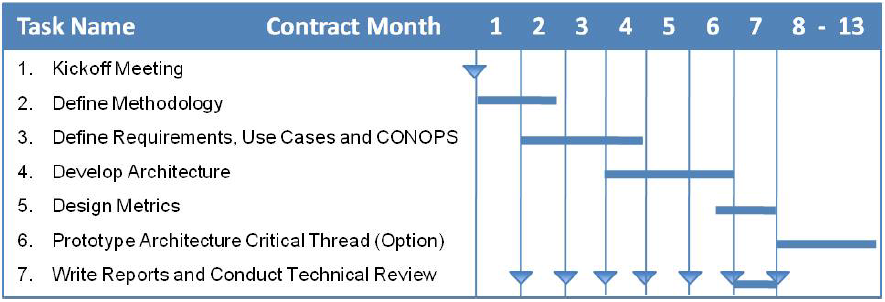
\includegraphics[width=5in]{./images/Gantt.png}}
 \caption{Task and milestone schedule.}
 \label{Gantt}
\end{figure}

\paragraph{Deliverables}
\begin{enumerate}[label=\alph*.] 
\vspace{-0.1in}
\item Kickoff meeting within 30 days of contract start.
\item Progress reports.
\item Technical review within 6 months.
\item Final report with SF 298.
\end{enumerate}

%Our work plan is fully responsive to the requirements stated in the AF131-039 topic. By producing a working proof-of-concept prototype, we will in fact achieve more than the requirements of the topic.

\newpage
\lfoot{\color{LeTigre}\scshape{Proprietary}}
\chead{\color{LeTigre}\scshape{Proprietary}~\\ Topic No: \fromtopicnum}
\cfoot{\color{LeTigre}\vspace*{-1.25em}{\scshape\fromproposaltitle}~\\ \rm\thepage~\\ 
\it{Use or disclosure of data contained on this page is subject to the restriction on the first page of this volume.}}

\sbirsection{Phase I Work Plan}
{This Phase I SBIR will result in the definition of the GeoAID technical approach and a software prototype that demonstrates the key aspects of our approach. These results will be in sufficient detail to show proof-of-concept and demonstrate feasibility for the Phase II project and Phase III commercialization.}

\subsection{Key Aspects and Innovation}
Modus Operandi is an experienced and highly capable SBIR/STTR contractor with a proven record of thorough research and innovation, directed toward solving real problems. MO has been active for over a decade in researching the key technologies required in this effort. AHS Engineering Services has 15 years of experience in research and development activities, and its members have faculty affiliations with the University of New Mexico and the Informatics Research Group, which is highly experienced in the areas of information security and usage management. Our approach integrates proven existing technologies with new innovative approaches. The use and leverage of proven technology provides a sound foundation for our technical approach, reducing technical risk, and providing a platform for our key innovations.

\subsection{Task Summary and Schedule}
The proposed Phase I effort is organized into the tasks shown in the Figure~\ref{Gantt}. Work will be performed at MO's headquarters in Melbourne, Florida and at AHS facilities in Albuquerque, New Mexico.

\begin{center}
\fcolorbox{BlueSteel}{Magnum}{
\begin{minipage}[t]{0.9\textwidth}
\begin{itemize}[labelindent=2em,leftmargin=1.5em,label=$\checkmark$] 
\item Building on information usage management and cloud expertise.
\item Reusing secure cross-domain information-centric systems for data delivery.
\item Mobile-first approach guarantees application-level configurability.
\item Innovative peering approaches to dynamic information delivery needs.
\end{itemize}
\end{minipage}}
\end{center}

\subsection{Task Details and Technical Approach}
The MO team will follow an agile software development process for accomplishing the Phase I tasks detailed below. Agile software development is a group of software development methods based on iterative and incremental development, where requirements and solutions evolve through collaboration between self-organizing, cross-functional teams. It promotes adaptive planning, evolutionary development and delivery, a time-boxed iterative approach, and encourages rapid and flexible response to change. It is a conceptual framework that promotes foreseen interactions throughout the development cycle, with a focus on delivering working software~\cite{La:03}.

\heading{Task 1: Kickoff Meeting}
We will hold a kickoff meeting either at the government's site or at MO headquarters, in Melbourne, Florida, based on Government Sponsor POC preference. In this meeting we will review the proposed technical approach and statement of work and clarify the research sponsor's technical direction. In order to begin to address specific system needs, the team will assemble a coarsely grained Concept of Operations document that describes how the GeoAID system should work. This will be a living document and will be updated regularly according to the agile process while the team executes other specific tasks. 

\heading{Task 2: Requirements Extraction}
The GeoAID system has a wide requirements domain, stretching from dynamic information usage management, to data storage, to message delivery schemes. In this task, we will identify and enumerate system requirements, aiming for 90\% requirements coverage overall and 100\% requirements coverage with respect to core Phase I functionality. We will name and describe these requirements in a form suitable for future system development and documentation. This analysis will include identification of Sponsor POC geospatial technology that should be used in future tasking.

The primary deliverable from this task will be a document describing these requirements such that the requirements can be traced both forward into the actual system and backward to the initial requirements source. The requirements will be enumerated as well as presented in either use case or user story formats.

\heading{Task 3: Establish Approaches and Architectures}
Capturing nodes suitable for broadcast is a difficult, nuanced problem. A variety of established architectural patterns can be potentially brought to bear on the problem, but they need to be carefully evaluated to ensure they will provide the required levels of service and scalability. In this task, we will outline the potential architectural approaches we can use, describe how and why they are applicable, and address how they could be evaluated for potential production use. We will leverage our established usage management technologies and experience to control information flow based on dynamic environmental context and the devices in use, extending that technology to seamlessly fit within this specific domain~\cite{JaLaHe:11,JaLaHe:12}.

This task will result in the development of a catalog of architectural options including descriptions of the approaches and their advantages and disadvantages. This catalog will also include specific evaluation points and potential proofs-of-concept that may be built into the GeoAID system.

\heading{Task 4: Evaluate System Architecture Options}
Building on the catalog established in the previous tasks, we will evaluate outlined technical and architectural approaches with an eye towards identifying common features. We will examine the options available to us and choose the most promising as well as determine how we can establish a common extensible framework for GeoAID in which we can instantiate components embodying various different approaches for future experimentation and comparison.

The outcome of this task is an ordered listing of potential approaches and an architectural outline of a common framework for GeoAID in which we can test the approaches identified.

\heading{Task 5: System Development}
In this task we will build a simple GeoAID framework based on the common architecture identified previously. We will keep the framework as simple as possible, but relevant and applicable to the operational domain. We will also develop components embodying the varied approaches to node capture, information usage management, and information dissemination. We will verify that these components can be loaded into the common GeoAID framework and run as expected so as to ease transition into future evaluation tasks. 

We will further build upon our cloud engineering experience and in-house infrastructure to develop economical, standards-based systems based around portable system configurations. This will include automating event collection for future reporting using systems deployed in our previous information-centric data flow research~\cite{LaHe:12b}. 

At the completion of this task we will have source code available that is capable of loading the operational components on demand, as specified by previously identified configuration primitives. We will be able to load and run this system using accepted geospatial displays identified in previous tasks with the help of the Sponsor POC.

\heading{Task 6: System Evaluation}
At this point in the project, we will have established the key GeoAID system components, developed the initial proof-of-concept technology, and will be prepared to evaluate various approaches and techniques to geographically-aware assumed information dissemination. Thus, in this task we will run the system and collect experimental results. During these experiments we will measure key performance attributes related to supportable system load, information delivery times, dropped messages, and appropriate message delivery. 

\heading{Task 7: Technical Review Meeting}
We will hold a technical review meeting with the Government Sponsor POC within 6 months of project commencement. The GeoAID concept of operations, system requirements, and architectural options will be reviewed and refined at this meeting.

\heading{Task 8: Proof-of-Concept Prototype}
We will develop a preliminary version of the GeoAID system as a proof-of-concept prototype demonstration. We will provide the demonstration using an accepted geospatial display from Sponsor POC recommended system(s), along with the software, design documents, test suites, and other supporting documentation.

\heading{Task 9: Reports and Publications}
We will prepare monthly progress reports, the final technical report with SF 298, and the non-proprietary summary report, including all pertinent observations, nature of problems, positive as well as negative results, and design criteria established. We envision that one or more professional conference and journal papers will result from this research. With the customer's approval, we will publish the research results.

The tasks outlined within this proposal identify specific deliverables the team will develop and submit to sponsoring organizations. Those specific deliverables include:

\begin{itemize}
\item {\bf Requirements}---A document listing identified requirements associated with requirement source organized both by list and context via use cases or user stories.
\item {\bf Architectural Catalog}---A document describing system architectural options, advantages and disadvantages of those options, and how the they can be evaluated.
\item {\bf Software Source Code}---Any and all developed source code, including proofs-of-concept and operational software. This will also include documentation of the developed software.
\item {\bf Automated Test Suite}---An automated test suite covering the system and all developed source code upon which the system is based.
\item {\bf Operational System}---The operational system itself. This will consist of operating system images, source code, and deployment instructions, as applicable.
\item {\bf Final Technical Report}---A report detailing the specifics of architectural evaluation activities, including information with respect to how the system operates, explanation of any design decisions made with supporting evidence, and guidance for future phase II activities.
\end{itemize}

\sbirsection{Related Work}{
Modus Operandi is highly qualified to successfully perform this effort based on our years of directly related experience in semantic technologies, data fusion, DoD Intelligence, Surveillance, and Reconnaissance (ISR) systems, and with enabling technologies such as service-oriented architecture and net-centric computing. AHS Engineering Services and the University of New Mexico's Informatics Lab are renowned for research in information security, information theory, and machine learning.}

\subsection{Co-Principal Investigators' Related Experience}
We propose Dr. Mark Heileman as MO's Phase I Co-Principal Investigator (Co-PI). Dr. Heileman has extensive experience as a research engineer and software system developer. His technological work has focused on applying artificial intelligence techniques and computer modeling to solve real-world business problems. Some of his early work in this area involved the practical application of expert systems and simulation modeling. More recently his work has involved the development of a trust evaluation framework for use in a layered sensing architecture that is intended to produce actionable situational awareness (the notion of trusted sensing is then built into the layered sensing architecture)~\cite{HeHeFiSt:09,HeHeHw:09}. He is currently the Co-PI on both the SMASHUP Phase II SBIR project and the Nublu Phase I STTR project. The SMASHUP research project will result in the development of a formal framework that allows integration via mashups of content from various data sources in a secure manner~\cite{HeHeGiEv:10,HeHeShGiJa:11}. The Nublu research project will deliver technological innovations to provide assured information sharing (AIS) capabilities using flexible cloud computing based architectures~\cite{HeHeNaLa:12}. A summary r\'esum\'e for Dr. Mark Heileman is provided in Section~\ref{MDH}.

We propose Dr. Gregory Heileman as AHS's Phase I Co-PI. Dr. Heileman has over twenty years of experience as a research scientist, and has published over one-hundred peer-reviewed journal articles and conference papers. His research interests are in the areas of information security and multimedia systems, the theory of computing and information, and machine learning. He serves on the Editorial Board for the International Journal of Multimedia Intelligence and Security. Dr. Gregory Heileman is considered an authority on information security and usage management ~\cite{Informatics}. Some of his early work in information security dealt with the development of secure container technology at the hardware level (see US Patent 6,731,756) \cite{PiHe:04}. His subsequent work has involved the development of architectural frameworks in support of access and usage control technologies \cite{HeJa:05,HeJaKhHr:07,JaHe:04,JaHeMa:06}, information forensics \cite{PeHeAb:07,QuPeHe:09}, and semantics-based information valuation \cite{AlHe:10,AlHe:08}. He is currently the Co-PI on the SMASHUP Phase II SBIR project and the Nublu Phase I STTR project; he will be a Co-PI on the ASW F2F Phase II STTR project. Dr. Gregory Heileman's experience is listed in Section~\ref{subs}.

\subsection{Modus Operandi Related Work}
Modus Operandi, Inc., is an advanced software technology firm serving the defense and intelligence community. We are focused on the development and marketing of technology and solutions that speed information discovery, integration, and fusion. We combine innovative semantic technology with defense sector software systems development experience in the Command, Control, Communications, Computers, Intelligence, Surveillance, and Reconnaissance (C4ISR) domain.

MO's R\&D focus is semantic web technologies with emphasis on semantic enrichment of multi-source data, intelligence fusion, unstructured information, reasoning, semantic integration, and migration of legacy systems to SOA. MO has deep expertise in text analytics, knowledge modeling and reasoning with heavy emphasis on open standards such as Extensible Markup Language (XML), XML Query Language (XQuery), Resource Description Framework (RDF), SPARQL (recursive acronym for SPARQL Protocol and RDF Query Language),Web Ontology Language (OWL), and other semantic Web technologies. We pride ourselves on being a service-oriented company, adapting our wide background of in-depth experience to solve an extensive range of customer problems relating to information discovery and exploitation.

\subsubsection{Related Work -- Corporate R\&D and Phase III Commercialization}
{\bfseries Wave Exploitation Framework Technology Portfolio}---MO employs a portfolio commercialization strategy under a single brand, called Wave-EF, to achieve maximum payback for our investment in product management, marketing, and sales. An overarching portfolio roadmap and architecture integrates contributions from numerous SBIR/STTR projects, commercialization partners, and internal R\&D efforts. Wave-EF components are targeted at the challenges of processing multi-source intelligence for intelligence exploitation. Wave-EF performs ``semantic enrichment'' via text analysis and machine reasoning within a scalable, component-based architecture.

\subsubsection{Related Work -- Research \& Development}\label{MO-related}
Summarized below are the R\&D projects conducted by MO that address the critical technologies that will enable successful GeoAID R\&D.

{\bf Green Wave: Assuring Trust between the Edges Phase I SBIR}---This project dealt with the problem of delivering universal situational awareness to decision makers, and in particular with the problem of providing a means of quantifying the ``goodness'' of the various pieces of information contained within a layered sensing framework. Layered sensing is characterized by the appropriate sensor or combination of sensors/platforms, infrastructure and exploitation capabilities to generate that situation awareness and directly support delivery of ``tailored effects.'' During this research effort we created prototype architecture that supported the gathering and propagating (both forwards, for decision making, and backwards, for post mortem analyses) of ``trust information'' computed at various nodes in a network. In addition, we computed trust metrics from this information that could be provided to a decision maker. \emph{Contract Completed January 2009. Customer: AFRL/RYTC, Mr. Jong Hwang. (937) 255-4709 x3591}.

{\bf SMASHUP: A Formal Framework for Secure Mashups Phase II SBIR}---The recent development of mashup technologies now enables users to easily collect, integrate, and display data from a vast array of different information sources available on the Internet. The ability to harness and leverage information in this manner provides a powerful means for discovering links between information, and greatly enhances decision-making capabilities. The availability of such services in a DoD environment will provide tremendous advantages to the decision-makers engaged in analysis of critical situations, rapid-response, and long-term planning scenarios. In this research project, we have developed a framework that will allow integration via mashups of content from various data sources in a secure manner. The framework is based on mathematical logic wherein data units are wrapped in policies that provide rules over the manner in which information is collected, aggregated, and rendered in different environments. An advantage of this approach is it provides a formal means for controlling the usage of resources within highly complex secure mashups. \emph{Current Contract Awarded May 2011. Customer: AFRL/RIEBB, Mr. Matthew Shaver. (315) 330-3295}.

{\bf Nublu: Assured Information Sharing in Clouds Phase I STTR}---We are developing an assured information sharing framework for cloud-based systems that leverages our ongoing work in the areas of policy-based usage management and semantic interoperability. The development of this framework will involve the creation of a novel approach to information sharing that treats security as a commodity that can be dynamically provisioned within the cloud, along with other cloud resources. Currently, the security of networked infrastructures tends to be managed statically. That is, security requirements are developed and implemented within the networking environment, and all of the information that traverses the network will have these hard-coded security policies applied to it. The research project addresses this issue by logically separating security policies from security implementations within the network. This approach is vital if the true capabilities of the cloud are to be realized in DoD environments; it naturally meshes with the philosophy behind cloud computing. Specifically, the main advantage of cloud systems is the automatic provisioning of resources according to current demands. In a DoD setting there will be multiple missions currently interacting with the cloud infrastructure, and the proposed framework will allow each mission to do so according to the current security demands. \emph{Phase II Contract Pending Award. Customer: AFRL/RITB, Ms. Virginia Ross. (315) 330-4384}.

{\bf Anti-Submarine Warfare Find-to-Forecast Phase I STTR}---The ASW F2F Project is focused on extracting situational knowledge from unstructured data sources, specifically tactical communications between Seahawk helicopters and the carrier, to fuse with structured data, such as radar and sonar data. This has involved developing a mission ontology for ASW, building a vocabulary for missions, and building specialized grammars for text parsing, tagging, extraction, and normalization as RDF triples. Phase I Contract awarded June 2011. \emph{Phase II Contract Pending Award. Customer: Office of Naval Research, Mr. David McGrane (360) 315-3531}.

\subsubsection{Related Work -- Technology Transition, Deployment, and Commercialization Opportunities}
This section summarizes the technology transition, deployment, and commercialization opportunities for Modus Operandi efforts relevant to the GeoAID project. Commercialization Partners are discussed in Section~\ref{commercialization}.

{\bf WebTHREADS}---MO's Wave text analytics and correlation technologies were integrated into the Web-based Threat HUMINT Reporting Evaluation Analysis and Display System (WebTHREADS), a web-based system for identifying and classifying intelligence reports used by Air Force organizations including the National Air and Space Intelligence Center (NASIC). Wave-EF uses domain-specific vocabularies, grammars, and ontologies to extract fourteen essential elements of information found in military intelligence reports, such as high-value individuals, locations, or events. MO also developed a tool for measuring the effectiveness of knowledge extraction from text, based on a standard text analysis metric, called F Factor Analysis. \emph{Contract Completed December 2010. Customer: Air Force Electronic Systems Center, 630th Electronic Systems Squadron, Jonathon L. Cozad,  Lt USAF, (781) 266-0869}.

{\bf Air Force ISR Agency Semantic Analysis Tool (SAT)}---The AF ISR Agency sought to inject new technology for enhanced exploitation of multiple sources of unstructured data [further details classified]. \emph{Contract completed December 2010. Customer: AF ISR Agency, Mr. John Gormaley (321) 494-0527}.

{\bf DCGS MC Multi-INT Semantics}---On this US Marine Corps project, Modus Operandi leveraged Wave-EF technology to build a DIB-enabled semantic wiki called Tactipedia. Tactipedia provides analysts with semantically integrated, mission-relevant information extracted from text sources. Links among pages (or semantic content) is based on semantic relations within an ontology, rather than hard-wired hyperlinks. In this way, Tactipedia's semantic model drives meaningful content integration as well as presentation to users. \emph{Phase II enhancement completed November 2011. Customer: USMC LtCOL Scott Camden, (703) 221-0200}.

\subsection{AHS Engineering Services Related Work}
Summarized below are the research projects conducted by AHS Engineering Services and the Informatics Research Laboratory at UNM that address the critical technologies that will enable successful GeoAID R\&D. As all aspects of science and society become increasingly information intensive, the need to understand, create, and apply new methods for modeling, managing, and acquiring information has never been greater. The UNM Informatics Lab, established by Professor Gregory Heileman, has considerable knowledge in the areas of information security, the theory of information, and information architectures.

{\bf Information Security/Security in Mashups. Project Name: ``SMASHUP: A Formal Framework for Secure Mashups,'' Phase II SBIR}, in collaboration with Modus Operandi, Inc., Melbourne, FL. See Section~\ref{MO-related} for project description.

{\bf Information Security in Clouds. Project Name: ``Nublu: Assured Information Sharing in Clouds,'' Phase I STTR} , in collaboration with Modus Operandi, Inc., Melbourne, FL. See Section~\ref{MO-related} for project description.

{\bf Network Architecture and Security. Project Name: ``Collaborative Research: Transient Network Architecture,'' National Science Foundation} in collaboration with the Center for National Research Initiatives (CNRI), Reston, VA. This work involved the development of the Transient Network Architecture for the next generation Internet. Our work on this project involved investigating how the capabilities offered by the networking architecture would facilitate the management of content. Specifically, we considered how the rights expressed by rights expression languages (RELs) could be supported by emerging Internet infrastructures. We considered how the ability to effectively use RELs could be further supported by changes made to the Internet infrastructure. For example, the notion of adding ``rights awareness'' to routers and firewalls was considered, allowing rights models to be more effectively and less intrusively implemented within the infrastructure. In addition, we addressed the problem of location-based rights in current and future infrastructures. This involved the consideration of authorized domains that essentially use the IP addresses of machines in order to determine where the content can be used, along with a more natural implementation of this problem that used handles as identifiers. \emph{Project completed July 2008. National Science Foundation, Future Internet Design (FIND) Program, Darleen Fisher, (703) 292-8950.}

\subsection{State of the Art Related Work}
The term \emph{usage management}, coined by the Key Personnel~\cite{JaHeLa:10}, is used throughout this proposal to refer to the process of managing how various resources are allowed to be used, manipulated, and processed within and across computing environments according to specified policy. This definition is very broad and encompasses many existing areas of information security and trustworthy computing. Figure~\ref{UM} provides a high-level view of the primary elements supporting the core capabilities of a usage management framework. We can think of usage management as a concept that unifies access control, usage control, along with digital rights management~(DRM), and enforcement mechanisms.
\begin{figure}
  \centerline{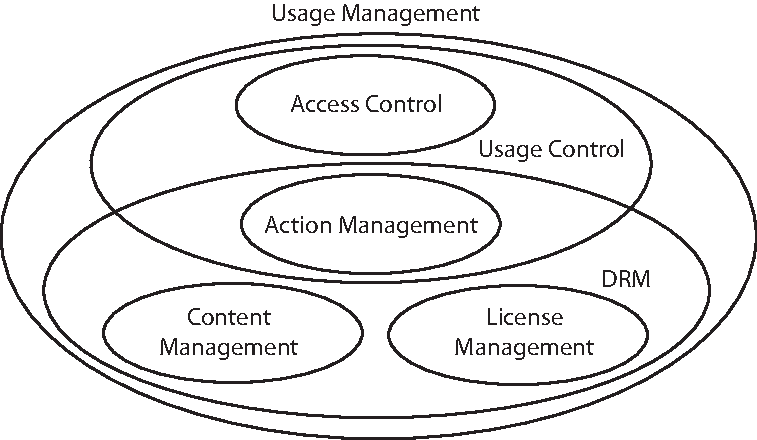
\includegraphics[width=3.5in]{./images/usage_management.pdf}}
  \caption{The primary elements associated with a usage management system.}\label{UM}
\end{figure}

\emph{Access control} by itself is a rudimentary form of usage management that is concerned with mechanisms for determining what subjects may access a given set of objects under what conditions. Over the years, access control policy models and supporting languages have continued to evolve with increasing granularity in policy expression and sophistication in reasoning power~\cite{BlPa:76,HuFeKu:06}. Usage control is a relatively new concept that incorporates access as well as usage policies for users over resources~\cite{PaSa:04}. \emph{Usage control} mechanisms focus on access and subsequent usage of a resource over a finite period of time. Usage control models take into account semantics such as obligations and permissions. One of the important distinguishing features of usage control is usage tracking. \emph{DRM} includes license (or policy) management, content management, tracking, negotiation, rights expression languages, and payments~\cite{HeJaKhHr:07,JaHe:08b,JaHeMa:06}. In general, in DRM systems, the use of content objects is subject to the terms of a license~(policy), which is expressed using a REL. The last major component of a usage management system involves \emph{enforcement mechanisms}. These include software and/or hardware mechanism that may be used in an effort to enforce usage according to specified policy.

These four areas form the components of a usage management system. A usage management system is thus capable of expressing complex, fine-grained usage policies over data elements and of ensuring subsequent interpretation, enforcement, and reasoning of these policies along with tracking of usage of those data elements in the computing environment. In this research, a usage management system will be developed specifically for the purpose of managing location-based policies and scenarios. 

The current state-of-the-art in location services for mobile device divides into a few distinct categories. First, there is geolocation of mobile devices based upon their IP addresses. These approaches use tables of IP address ranges and other associated information to provide location services to subscribers via regional Internet registries~\cite{AIRN:13,RIPE:13}. This information can be retrieved via standard programming interfaces defined by the World Wide Web Consortium (W3C)~\cite{w3c:13}, and are supported by a variety of browser implementations ~\cite{firefox:13,Pi:13}. With this approach, developers use standard interfaces to retrieve information from Internet registries in order to locate individuals. This type of functionality exists for modern browsers on workstation-grade systems, as well as on most mobile platforms~\cite{opera:13,safari:13}.

Another approach involves the use of dedicated GPS systems with network links. These types of systems are embodied by various platform mapping applications common on mobile platforms~\cite{amap:13,gmap:13}. Apple's iPhone, for example, currently offers assisted GPS services that use GPS information transmitted from satellites, as well as cellular and other network sources to locate devices~\cite{amap:13}. Though any of these systems can be used in device-to-device communication in a distributed Internet-of-things, GPS-equipped units are more common as they can provide finer levels of geolocation granularity.

Finally, bringing this information together, there are data solutions such as those embodied by Google Earth and Esri %do not capitalize this!
products such as ArcGIS~\cite{esri:13,gearth:13}. Both GPS-based and IP address-centric geolocation techniques can integrate with these types of data solutions into a single, unified system. With that in mind, however, these kinds of geographic information systems do not provide messaging functionality directly, nor do they implicitly support it---they can be leveraged as components to provide integrated solutions.

\sbirsection{Relationship with Future Research or Research and Development}{}
Modus Operandi was founded to address the practical application of innovative technologies. As a result, we are committed to the approach described in this proposal and are enthusiastic about its potential. The results of this program will have a significant influence on the future R\&D performed by Modus Operandi. Our current and past R\&D projects and our ongoing Wave technology development provide an excellent technical foundation for the Phase I effort. Phase I will demonstrate the feasibility of our approach and will lay the groundwork for the Phase II development and transition. Specifically, upon successful completion of Phase I, we will have: (1) identified the critical aspects of our technical approach, (2) demonstrated the proof-of-concept, and (3) constructed a roadmap for application to Air Force initiatives such as High Frequency Global Communications System (HF-GCS), which includes identifying the applicable clearances, certifications, and approvals required to conduct Phase II testing. Collectively, the anticipated results from Phase I will provide a solid foundation for Phase II. In Phase II, we will build the full GeoAID framework and apply it to the HF-GCS. Phase III would bring this GeoAID framework to the marketplace (see Section~\ref{commercialization} below).

Our successful realization of our Phase I and II objectives and achievement of Phase III commercialization is expected to provide the following benefits to both Government and private sector customers of GeoAID:
\begin{itemize}
     \item Dynamically and securely share information with properly credentialed users based upon location.
     \item An agile usage management framework that scales to the enterprise.
     \item Provides an information advantage to warfighters.
\end{itemize}
We are confident of our ability to successfully deliver these benefits. As for future R\&D, we will seek out ways to extend the scope of GeoAID to include more sophisticated policy-based usage management capabilities.

\sbirsection{Commercialization Strategy}{Our overall strategy for achieving technology transition and commercialization success will be to position GeoAID as a high-value enhancement to our Wave product and related services, thereby leveraging our existing commercialization momentum and resources. Our three-pronged approach to achieving this strategy is to: (1) transition the GeoAID technology to HF-GCS, (2) deploy the technology to our other existing defense sector customers, and (3) leverage partnerships with prime contractors and commercial software vendors as channels for broader commercialization. Our overall goal is to build a profitable line-of-business while providing high return-on-investment to our Air Force transition customers.}
\label{commercialization}
\paragraph{Phase III Success Indicators:} 
\begin{center}
\vspace{-12pt}
   \fcolorbox{BlueSteel}{Magnum}{
         \begin{minipage}[t]{0.9\textwidth}
             \begin{itemize}[labelindent=2em,leftmargin=1.5em,label=$\checkmark$] 
  		\item SBIR/STTR Commercialization Achievement Index (CAI) of 90.
  		\item Annual corporate investment in commercialization initiatives exceeds \$1 million/year.
  		\item Winner of \$9.3M Phase III contract with Army CECOM in 2004 and \$9.9M Phase III in 2011.
  		\item Winner of U.S. Small Business Administration Tibbetts Award, recognizing our innovation, economic impact, and business achievements in the SBIR Program.
		\item Government prime contractor partnerships with Lockheed Martin, Northrop Grumman, ManTech, L-3 Communications, Booz Allen, SAIC, etc.
 	\end{itemize}
         \end{minipage}
      }
\end{center}

\paragraph{Background.} Modus Operandi's vision is to create solutions that speed information discovery, fusion, integration, and understanding. We combine innovative semantic technology with defense sector software systems development experience in the C4ISR domain. As demonstrated by our SBIR/STTR CAI of 90, we have a track record of successful technology commercialization, particularly with our Wave technology portfolio. Partly as a result of our SBIR/STTR commercialization and technology transfer efforts, our commercial (non-R\&D solutions for federal and private sector customers) business base has grown from less than 10\% to more than 60\% of our company's revenue. The following subsections provide our market analysis and plans for commercialization of GeoAID.

\paragraph{Commercialization Strategy.} Our experience has identified two keys to successful SBIR/STTR commercialization: (1) strategic synergy between the SBIR/STTR technology and our core business focus, and (2) strong Phase II/III partnerships.
This experience bodes well for the GeoAID project: first, because of GeoAID's direct tie with our strategic focus on serving the warfighter through innovative technology solutions for discovery, integration, and fusion of multi-source information; and second, because the proposed application of the technology directly addresses challenges faced by the Air Force; by our other defense sector customers (i.e., US Army, Marine Corps, NAVAIR, Strategic Operations Command, and Missile Defense Agency); and by our prime contractor (e.g., Northrop Grumman, Lockheed Martin, ManTech, SAIC) and commercial (e.g., Ultra Electronics, Franz, NutraSpace) partners.
Our strategy for GeoAID commercialization will be as an integral part of our Wave product line and associated services. We plan to pursue three paths to commercialization of GeoAID. All of these paths are already part of our Wave marketing program.
\begin{enumerate}
  \item Our first path focuses on transitioning the technology to the HF-GCS thereby providing direct ROI for AFRL SBIR investment. Our existing knowledge and experience working with the Air Force ISR Agency, the Electronic Systems Center, and the 45-th Space Wing will provide a solid foundation for success in this initiative.
  \item Our second path is deployment to our existing DoD customers and prime contractors, leveraging the GeoAID technology to address both known and anticipated needs they face in the area of machine learning and reasoning.
  \item The third path is expanding our business partnerships with prime contractors and commercial software vendors, increasing our market share in the federal sector, and ultimately taking us into the commercial marketplace. We are leveraging our partnership-building experiences to incorporate revenue channel and technology partnerships as a key element in our commercialization strategy.
\end{enumerate}

\paragraph{Market Need and Size.} Our commercialization strategy consists of two stages. We are currently focused on the first stage, which is establishing Modus Operandi as a premier niche technology solutions provider in the C4ISR market sector. The second stage will be to extend the business partnerships we develop in the first stage to package our Wave technology for the broader federal and commercial markets.

We are actively executing a comprehensive business plan which sets forth our strategy and roadmap for our technology, for delivering high value to customers, and for building a successful company. Our first stage market focus is on a niche within the \$16 billion C4ISR market~\cite{iCD:12}. Although overall defense-related spending is expected to flatten, and likely decline, over the next 10 years, the C4ISR market is projected for continued growth. The overall C4ISR segment is projected to grow at a compound annual growth rate of 2.98\% over the next decade~\cite{iCD:12}. This growth is fueled by the demand for timely intelligence as well as by technology and doctrine factors, particularly the demand for systems interoperability and the emergence of network-centric operations.

Within these overall market segments, relevant niche markets for Modus Operandi include Big Data, data discovery/integration/sharing, unstructured data analytics, multi-source intelligence analysis, and situational awareness, with concentration on the needs of U.S. DoD and intelligence community. Our preliminary estimate of the size of the MO-addressable portion of this market niche (comprised of R\&D, acquisition, and sustainment programs) is \$500-800 million annually.

\paragraph{Projected Commercialization Results.} Using our three-pronged strategy, we project achievement of the results shown in the Table~\ref{commercialization}. (Note: Our commercial market potential is not included, and offers the potential to significantly increase these estimates.)
\begin{table}
\begin{center}
 \caption{Actual and projected commercialization achievements.}\label{results}
 \begin{tabular}{|cccl|} \hline
  {\color{BlueSteel}\sf\bfseries\textsc Description}   &  {\color{BlueSteel}\sf\bfseries\textsc Timeframe} &    {\color{BlueSteel}\sf\bfseries\textsc Amount}  &  {\color{BlueSteel}\sf\bfseries\textsc Comments} \\ \hline
   Working Capital: 					& 						&						& Raised in April 2005 through sale \\ 
   Funds Raised					& 			2005			&		\$450M			& of non-core technology to a com-  \\
   Current Working Capital Assets		& 			2012			&		\$2M+			& mercial firm. Existing capital           \\
   								&						&						& resources. \\ \hline
   Customer Investments (USAF 45th		&						&						& \$4.6M customer/investor funds  \\
   Space Wing, AFRL, AFTAC, AF		&		2004-2012		&		\$7.6M			& and \$3M matching/add'l funds  \\
   ESC, Marine Corps, CECOM and		&						&						&  and CPP fund onrelated Phase II \\
   PEO IEW\&S)						&						&						& SBIRs with USAF and    Army.     \\ \hline
   Modus Operandi IR\&D Investment	&		2012-2015		& 		\$250K			& Estimated funds from additional \\
   								&						&						&  ModusOperandi IR\&D invest-    \\ 
								&						&						& ment. 						\\ \hline
   Additional Phase II/III 3rd-Party		&		2015-2016		&		\$2-3M			& Anticipated from early adopters         \\
   Investment						&						&						& and business partners.			\\ \hline
   Ramp-up Period Revenue			&		2016-2017		&	\$500K increasing 		& A 2-year ramp-up is projected. 		\\ 
   								&						& 	to \$3M annually		&							\\ \hline
   Full Scale Sales \& Marketing			&		2018 and 			& 	\$3+M annually			& Based on direct sales and co- \\
   								& 		beyond			&	out of \$20M total		& marketing initiatives. See          \\
								&						&						& assumptions below.	\\ \hline
 \end{tabular}
\end{center}
\vspace{-6pt}
{\small Key Assumptions: (1) Revenue includes both product licenses and related services. (2) MO participates as a partner in \$500 million of prime contractor/partner orders annually by 2018. (3) MO's revenue participation averages a minimum of 4\% (\$20 million annually by 2017). (4) The revenue share attributable to GeoAID is 15\% (\$3 million annually). (5) Excludes revenue from commercial markets.}
\end{table}

\sbirsection{Key Personnel}{Modus Operandi prides itself on teaming superbly qualified personnel for all of our projects. }
All key personnel are United States citizens. We propose Dr. Mark Heileman and Dr. Gregory Heileman as Phase I Co-Principal Investigators. Dr. Mark Heileman's biography and r\'esum\'e are below. Dr. Gregory Heileman's biography and r\'esum\'e are in Section~\ref{subs}.
\begin{center}
   \fcolorbox{BlueSteel}{Magnum}{
         \begin{minipage}[t]{0.9\textwidth}
             \begin{itemize}[labelindent=2em,leftmargin=1.5em,label=$\checkmark$] 
  		\item Dr. Mark Heileman has extensive experience as a research engineer and software system developer. He has focused on applying advanced information technology and modeling to solve real-world business problems.
  		\item Dr. Gregory Heileman is a recognized leader in machine learning and directs the Informatics Lab at the University of New Mexico where he is Associate Provost and Professor in the Department of Electrical and Computer Engineering.
		\item Dr. Christopher Lamb  is a TOGAF certified enterprise architect and software engineer with nearly two decades of experience building software systems. He is actively engaged in cyber-security research as well, focusing specifically on distributed content network topologies, usage management, and cloud computing.
 	\end{itemize}
         \end{minipage}
      }
\end{center}

\vspace{-6pt}
\subsection{Modus Operandi Key Personnel Biography}\label{MDH}
{\bfseries Co-Principal Investigator. Dr. Mark Heileman} is a Senior Scientist at Modus Operandi. Dr. Heileman's over thirty-year career includes engineering and executive positions with Elisar Software Corporation, i2 Technologies, United Space Alliance, Rockwell International, and Harris Corporation. His mission is to focus on the client's challenges and employ a consultative, systems engineering approach to solve complex business needs. Dr. Heileman is a graduate of the University of Central Florida where he earned a Ph.D. in Industrial Engineering and Management Systems. He is a registered professional engineer in Florida.

\subsection{Co-Principal Investigator R\'esum\'e}
\textbf{\textsc{Mark D. Heileman \hfill Senior Scientist}}

\vspace{-18pt}
{\textcolor{black}{\makebox[6.5in]{\hrulefill}} 
\textbf{\textsc{Technical Expertise:}}
\vspace{-8pt}
\begin{multicols}{2}
 \begin{itemize}
  \item Enterprise Information Systems
  \item Digital Rights Management
  \item Cyber Security
  \item Expert Systems
  \item Data Aggregation
  \item Simulation and modeling	
 \end{itemize}
\end{multicols}
\vspace{-16pt}
\textbf{\textsc{Selected Publications:}}
\vspace{-8pt}
\begin{enumerate}
\item M. Heileman, G. Heileman, M. Shaver, P. Jamkhedkar, and M. Gilger. SMASHUP: Secure Mashup for Defense Transformation and Net-Centric Systems. Prepared for SPIE Defense, Security, and Sensing 2011 Conference, Orlando, FL, 25--29 April 2011.
\item G. Heileman and M. Heileman. Method and Apparatus for Integrating Subjective Trust Measures into Automated Decision-Making Processes. Provisional Patent Application, USA, submitted 19 May 2010.
\item M. Heileman, G. Heileman, and J. Hwang. Integrating Subjective Trust into Networked Infrastructures. Prepared for Systems \& Software Technology Conference (SSTC) 2009, Salt Lake City, UT, 20--23 April 2009.
Hull, R., K. Bimson, M. Heileman, R. Hyle, and R. Thiebauth. Semantic Service-Oriented Architecture for Range Operations: Evolving the Role of Semantics in the Enterprise. Prepared for SPIE Defense, Security, and Sensing 2009 Conference, Orlando, FL, 13--17 April 2009.
\item H. Goldstein, G. Heileman, M. Heileman, et al. Protecting Digital Archives at the Greek Orthodox Archdiocese of America. Prepared for DRM'03, Washington, DC, 27 October 2003.
\item D. Linton, S. Khajenoori, M. Heileman, J. Bullington, H. Cat, K. Halder, G. Hebert, and S. Sinnappan. ``Reporter Object: An Analysis Module Which Aids in Verifying, Validating and Graphically Displaying Results of Simulation Models,'' Simulation, Vol. 62, No. 5, May 1994, pp. 313--328.
\item M. Heileman, D. Linton, and S. Khajenoori. ``Simulation Study Aids Space Shuttle Flight Rate Planning,'' Industrial Engineering, Vol. 24, No. 3, March 1992, pp. 58--59.
\end{enumerate}

\vspace{-6pt}
\textbf{\textsc{Relevant Experience:}}~\\
{\bfseries Modus Operandi, Inc., 2004--present. Senior Scientist.} A software company serving the US defense and intelligence community by providing technology to speed information discovery, integration, and fusion. Directs the design and development of innovative information system technologies and their application to government and industry needs.~\\
{\bfseries Elisar Software Corporation, 2001--2003. Vice President, Sales Engineering.} A venture capital financed start-up software company providing digital rights enforcement products and services. Initiated the Sales Engineering function, which had primary responsibility for driving customer and market requirements into the internal development process.~\\
{\bfseries i2 Technologies, 1997--2001. Senior Solution Consultant}. A business software and services company providing supply chain management solutions to customers worldwide. Provided technical leadership throughout software products sales cycles.

\vspace{-6pt}
\textbf{\textsc{Education:}}
\vspace{-30pt}
\begin{tabbing}*****************\=\kill
 \> {\bfseries Ph.D.}, Industrial Engineering \& Management Systems, Univ. of Central Florida (1997). \\
 \> {\bfseries M.S.}, Engineering Management, Florida Institute of Technology (1990). \\
 \> {\bfseries M.B.A.}, Business Administration, Florida Institute of Technology (1985). \\
 \> {\bfseries B.S.}, Industrial and Systems Engineering, University of Florida (1980).
\end{tabbing}

\vspace{-12pt}
\textbf{\textsc{Affiliations:}}
\vspace{-30pt}
\begin{tabbing}*****************\=\kill
\> Registered Professional Engineer, State of Florida (P.E. \#35539). \\
\> Senior Member, Institute of Industrial Engineers. \\
\> Member, International Council on Systems Engineering (INCOSE). \\
\> Security Clearance: DoD Top Secret/SCI/SI/TK/G/HCS.
\end{tabbing}
\vspace{-12pt}

\sbirsection{Foreign Citizens}{}
We do not expect to involve any foreign citizens on this project.

\sbirsection{Facilities/Equipment} {}
All instrumentation and physical facilities required to carry out the Phase I effort are available at the Modus Operandi headquarters in Melbourne, Florida and at the AHS Engineering Services facilities in Albuquerque, NM. MO's 14,500 sq. ft. facility has a fiber optic Internet connection with a dedicated 4-Mbit bandwidth. Engineering laboratories host shared and project-dedicated resources, including two labs dedicated to classified work at the Secret level. These facilities meet all environmental laws and regulations of federal, Florida, and local governments for, but not limited to, the following groupings: airborne emissions, waterborne effluents, external radiation levels, outdoor noise, solid and bulk waste disposal practices, and handling and storage of toxic and hazardous materials.

\sbirsection{Subcontractors/Consultants}{Dr. Gregory Heileman and Dr. Chris Lamb are uniquely qualified for this effort, and their active involvement will ensure the success in delivering value to the Air Force Research Laboratory.}\label{subs}

\subsection{AHS Engineering Services Key Personnel Biography}\label{AHS}

{\bf Co-Principal Investigator. Dr. Gregory Heileman } is the Associate Provost for Curriculum and a Professor in the Department of Electrical and Computer Engineering at the University of New Mexico, with over 20 years of experience as a research scientist, and over 100 peer-reviewed journal articles and conference papers. At the University of New Mexico he teaches courses in the areas of algorithms and data structures, software design, theory of computing, learning theory, and information theory. His research interests are in the areas of information security and multimedia systems, the theory of computing and information, and machine learning. He currently serves on the Editorial Board for the International Journal of Multimedia Intelligence and Security. He is the author of the textbook Data Structures, Algorithms, and Object-Oriented Programming published by McGraw-Hill in 1996. During 1998 he held a research fellowship at the Universidad Carlos III de Madrid, and in 2005 he held a similar position at the Universidad Polit\'enica de Madrid. Dr. Heileman is a senior member of the IEEE. He holds a PhD in Computer Engineering from the University of Central Florida.

\vspace{-8pt}
{\bf Senior Scientist. Dr. Christopher Lamb} will act as the primary Systems Architect during the course of all phases of the project. Dr. Lamb currently serves as an Enterprise Architect, with concentration on Systems and Security, with Sandia National Laboratories. He is also a research professor affiliated with the Electrical and Computer Engineering department at the University of New Mexico. He has extensive experience designing and developing mission-critical distributed systems for a wide range of government departments and agencies. Prior to joining Sandia National Laboratories, Dr. Lamb served in executive roles and as a principal consultant for a variety of technology companies in the southwest. Dr. Lamb has a B.S. in Mechanical Engineering from New Mexico State University, an M.S. in Computer Science from the University of New Mexico, as well as a Ph.D. in Computer Engineering with a focus on Computational Intelligence from the University of New Mexico. He is a The Open Group Architecture Framework (TOGAF) 9 Certified Enterprise Architect and a Certified Information Systems Security Professional (CISSP) through the International Information Systems Security Certification Consortium.

\subsection{Co-Principal Investigator R\'esum\'e}\label{GLH}

\textbf{\textsc{Gregory L. Heileman \hfill Professor and Associate Provost}}

\vspace{-18pt}
{\textcolor{black}{\makebox[6.5in]{\hrulefill}} 
\textbf{\textsc{Technical Expertise:}}
\vspace{-8pt}
\begin{multicols}{2}
 \begin{itemize}
  \item Machine Learning
  \item Usage Management
  \item Information Security
  \item Data Structures and Algorithmic Analysis
  \item Theory of Computing and Information	
 \end{itemize}
\end{multicols}

\vspace{-16pt}
\textbf{\textsc{Selected Publications:}}
\vspace{-8pt}
\begin{enumerate}
\item C.~C. Lamb and G.~L. Heileman. Content-centric Information Protection in the Cloud, {\sl International Journal of Cloud Computing and Services Science  (IJ-CLOSER)}, 2(1):246-257, 2013.
\item P. A. Jamkhedkar, C. C. Lamb, and G. L. Heileman. Usage Management in Cloud Computing, In F. Hartung, T. Kalker and S. Lian, Eds., {\sl Digital Rights Management: Technology, Standards and Applications}, Auerbach Publications, 2012. 
\item C. C. Lamb, P. A. Jamkhedkar, G. L. Heileman and C. T. Abdallah. Managed Control of Composite Cloud Systems. 6th IEEE International Conference on System of Systems Engineering (SoSE), Albuquerque, NM, pp. 167--172, June 27--30, 2011.
\item P.~A. Jamkhedkar and G.~L. Heileman. Rights Expression Languages, in S. Lian and Y. Zhang, Eds., {Handbook of Research on Secure Multimedia Distribution}, IGI Global, Hershey, PA, 2008. 
\item S. al-Saffar and G. L. Heileman. Computing Information Value from RDF Graph Properties. Proceedings of the 12th International Conference on Information Integration and Web-based Applications \& Services, Paris, Nov. 8--10, 2010.
\item T.-T. Quach F. Perez-Gonzalez, and G. L. Heileman. Model-Based Steganalysis Using Invariant Features. IS\&T/SPIE Electronic Imaging Science and Technology: Media Forensics and Security XI (Conference EI120), San Jose, CA, Jan. 18--22, 2009.
\item S. al-Saffar and G. L. Heileman. Semantic Impact Graphs for Information Valuation. Proceeding of the Eighth ACM Symposium on Document Engineering, Sao Paulo, Brazil, pp. 209--212, Sept. 16--19, 2008.
\item S. al-Saffar and G. L. Heileman. Semantics-Based Information Valuation. Proceedings of the 4-th IEEE International Conference on Intelligent Systems IS'08, Varna, Bulgaria, Vol. 1, pp. 6-51--6-58, Sept. 6--8, 2008.
\end{enumerate}

\vspace{-6pt}
\textbf{\textsc{Relevant Experience:}}~\\
{\bfseries AHS Engineering Services, 1997--present. Principal.} A consulting firm offering expert engineering services in areas including software engineering and information security.~\\
{\bfseries University of New Mexico, Department of Electrical \& Computer Engineering, 1990--present. Professor, Associate Provost for Curriculum (current position)}.~\\
{\bfseries Elisar Software Corporation, 2000--2003. Chief Executive Officer and Chairman of the Board.} A venture capital financed start-up software company providing digital rights enforcement products and services.

\vspace{-6pt}
\textbf{\textsc{Education:}}
\vspace{-30pt}
\begin{tabbing}*****************\=\kill
 \> {\bfseries Ph.D.}, Computer Engineering, University of Central Florida (1989). \\
 \> {\bfseries M.S.}, Biomedical Engineering \& Mathematics, University of North Carolina (1986). \\
 \> {\bfseries B.A.}, Biology, Wake Forest University (1982).
\end{tabbing}

\vspace{-12pt}
\textbf{\textsc{Affiliations:}}
\vspace{-30pt}
\begin{tabbing}*****************\=\kill
\> Editorial Board,  International Journal of Multimedia Intelligence and Security. \\
\> Senior Member, IEEE. \\
\> Security Clearance: DoD Secret.
\end{tabbing}
\vspace{-12pt}

\sbirsection{Prior, Current, or Pending Support of Similar Proposals or Awards}{}
No prior, current, or pending support for the proposed work.

{\small
 \bibliography{proposal}
 \bibliographystyle{abbrv}
 }
 
\end{document} 